\documentclass[showkeys, prb, reprint]{revtex4-1}
\usepackage{amsmath}
\usepackage{graphicx}
\usepackage{epstopdf}
\graphicspath{{figures/}}

%% New commands
\newcommand{\F}{\mathcal{F}}
\newcommand{\A}{\rho_A}
\newcommand{\B}{\rho_B}
\newcommand{\dd}{\mathrm{d}}
\renewcommand{\d}{\delta}
\renewcommand{\l}{\left}
\renewcommand{\r}{\right}
\newcommand{\f}{\frac}

\begin{document}

%% Front (Top really...) Matter

\title{Regular Binary Phase Field Crystal Model}
\author{Nathan Smith}
\affiliation{McGill Department of Physics}
\author{Nikolas Provatas}
\affiliation{McGill Department of Physics}
\date{\today}

\begin{abstract}

Modelling the liquid in a binary PFC model as regular solution instead of an ideal one leads to lots of interesting features. Look at all those features. We'll even discuss how it can be a contributor to non-classical nucleation pathways. Very sexy.

\end{abstract}

\keywords{nucleation, growth, phase field crystal}

\maketitle

%% Body

\section{Introduction}

\section{Free Energy Functional for Binary Alloys}

To construct a free energy functional for a binary alloy we begin by splitting the free energy into ideal and excess components.

\begin{equation}
	\mathcal{F}[\A, \B] = \F_{id}[\A, \B] + \F_{ex}[\A, \B]
\end{equation}
The ideal component of the free energy is derived from the non-interacting, kinetic part of the Hamiltonian while the excess component is derived from the interaction potential of the Hamiltonian. The ideal component can be computed exactly as, 

\begin{equation}
	\beta\F[\A, \B] = \sum_{i} \int \dd r\, \rho_i(r) \l(\ln\l(\Lambda_i^3\rho_i(r)\r) -1 \r)
\end{equation}
Where the sum runs over components, $A$ and $B$, and $\Lambda_i^3$ is the thermal de Broglie volume. The excess free energy cannot, in general, be computed exactly and thus approximate it by expanding the excess free energy about a uniform reference mixture with densities $\A^0$ and $\B^0$.

\begin{align}
	\beta\F_{ex}[\A, \B]  &= \beta \F_{ex}^0 + \int \dd r \, C_i^{(1)}(r) \d \rho_i(r) \\
		&+ \f{1}{2}\int \dd r\, \d \rho_i(r) \,C^{(2)}_{ij} \ast \d\rho_j  + ... \nonumber
\end{align}
Where, summation over repeated indices is implied and $\ast$ denotes a convolution. $C^{(n)}(r_1, r_2, ...r_n)$ denotes the n-point direct correlation function. We now perform a change a variable to solute concentration, $c$, and dimensionless total density, $n$.

\begin{gather}
	n = \f{\delta \rho}{\rho^0} = \f{\d \A + \d \B}{\A^0 + \B^0} \\
	c = \f{\B}{\A + \B}
\end{gather}
Under this change of variables, the ideal free energy separates cleanly into total density and ideal free energy of mixing term as we might expect.

\begin{gather}
	\f{\beta\F_{id}[n, c]}{\rho^0} = \int \dd r\, \l( \l(n + 1\r) \ln\l(n + 1\r) - n  
	 + \l(n + 1 \r) f_{mix}(c) \r)
\end{gather}
Where,

\begin{equation}
  f_{mix}(c) = c\ln\l(\f{c}{c_0}\r) + (1 - c)\ln\l(\f{1 - c}{1 - c_0}\r).
\end{equation}

If we assume that the concentration field varies over a much longer length scale than the pair correlation functions (typically several particle radii), we can approximate the excess term as follows,

\begin{align}
	\f{\beta \F_{ex}[n, c]}{\rho^0} = -&\f{1}{2} \int \dd r\, n \l( C_{nn} \ast n + C_{nc} \ast \d c\r) \nonumber \\
	- &\f{1}{2} \int\dd r\, \d c \l( C_{cn} \ast n + C_{cc} \ast \d c\r).
\end{align}
where the $n-c$ pair correlation functions are,

\begin{align}
	C_{nn} &= \rho_0 \l(c^2 C_{BB}^{(2)} + (1 - c)^2 C_{AA}^{(2)} + 2c\l(1 - c\r) C_{AB}^{(2)} \r) \\
	C_{nc} &= \rho_0 \l(c C_{BB}^{(2)} - (1-c)C_{AA}^{(2)} + (1 - 2c) C_{AB}^{(2)} \r)\\
	C_{cn} &= C_{nc} \\
	C_{cc} &= \rho_0 \l(C_{BB}^{(2)} + C_{AA}^{(2)} - 2C_{AB}^{(2)} \r)
\end{align}



\subsection{Simplified Regular Free Energy Functional}

Following Greenwood \textit{et al.} [cite!] we can now expand the ideal free energy about reference density in a Taylor expansion and coarse grain the excess contributions to the free energy. In contrast to Greenwood \textit{et al.}, we will not assume that the $k = 0$ mode of the effective concentration-concentration correlation is zero. The effect of eliminating this assumption is that two terms are now produced by performing a gradient expansion of $C_{cc}$.

\begin{equation}
	C^{c_0 c}_{eff}(r, r^\prime) = \delta(r - r^\prime)\l(\epsilon  - W_c \nabla^2 + ... \r)
\end{equation}

The first term serves to produce a free energy of mixing with a regular solution model instead of an ideal solution. That is to say, there is both an entropy \textit{and} enthalpy of mixing in the theory. Ultimately, the rest of the free energy looks the same as that of Greenwood,

\begin{align}
	\f{\beta \Delta \F[n, c]}{\rho_0} &= \int \d r \f{n^2}{2} - \eta \f{f^3}{6} + \chi \f{n^4}{12} -\f{1}{2} n C^{n}_{eff} \ast n \\
	&+ \int \d r \f{W_c}{2} \l\vert\nabla c\r\vert^2 + \omega (n + 1) f_{mix}(c) + \f{1}{2} \epsilon (c- c_0)^2, \nonumber
\end{align}

Where, $\eta$, $\chi$ and $\omega$ are fitting parameters. Hypothesizing a spinodal point in the liquid free energy at temperature $T_c$ we can model the temperature dependence of $\epsilon$ with a linear expansion about this point. 

\begin{equation}
	\epsilon(T) = \omega \l( -4 + \epsilon_0 \l(T - T_c\r)\r) 
\end{equation}

While the proposed adjustment seems minimal at face values, we'll that it allows for the modelling a broad spectrum of binary phenomena.

\subsection{Modelling Correlation Functions}

To model the density-density correlation function $C_{nn}(r)$ or equivalently, $\tilde{C}_{nn}(k)$ we function in the form of a sum of products of window functions, $\chi_i$, in concentration and structure functions, $\tilde{C}_i$, in Fourier space, 

\begin{equation}
  \tilde{C}_{nn}(k; c) = \sum_i \chi_i (c) \tilde{C}_i (k)
\end{equation}

This model reflects, qualitatively, the fact that different structures are stabilized at different concentrations. The window function $\chi_i$ decribes the region in concentration space over which a phase $i$ is stable and the structure function, $\tilde{C}_i$ describes the structure of that phase. The structure functions can be modelled by a sum of gaussians in fourier space, 

\begin{equation}
  \tilde{C}_i(k) = e^{T/T_0}\l(\sum_j e^{-\f{(k - k_j)^2}{2 \alpha_j^2}}\r).
\end{equation}


\subsection{Model Dynamics}

We can model the dynamics of the total density and concentration using diffusive, conservative dynamics for each. We'll further assume that the mobility of both concentration and total density are constant. 

\begin{gather}
	\f{\partial n}{\partial t} = M_{n} \nabla^2 \l[n - \eta \f{n^2}{2} + \chi \f{n^3}{3} + f_{mix}(c) - C^n_{eff} \ast n \r] + \nabla \cdot\xi_c, \\
	\f{\partial c}{\partial t} = M_{c} \nabla^2 \l[\l(\epsilon - \nabla^2\r)c + \l(n + 1\r)\f{\partial f_{mix}}{\partial c} - \f{1}{2} n \f{\partial C^n_{eff}}{\partial c} \ast n\r] + \nabla \cdot \xi_n.
\end{gather}

Where $\xi_c$ and $\xi_n$ are noise terms respecting a generalized Einstein relation. It is important to note that $c$ is in fact not a conserved variable but rather a ratio of conserved variables $\B$ and $\rho$. Therefore, these dynamics can only be considered valid in the limit where total density is constant (eg. these is no density segregation between phases) in addition to the constraints discussed by Fang [cite!]. 

\section{Equilibrium Properties}

Here, we'll explore the flexibility of our simplified regular model to describe previous and new classes of invariant reactions for the binary alloy.

\subsection{Eutectic Phase Diagram}

While previous PFC models have shown that elastic energy is a sufficient driving force for eutectic solidification our simplified regular model allows for the examination of the role enthalpy of mixing can play in eutectic solids. For instance, Murdoch and Schuh noted that in nanocrystalline binary alloys, while a positive enthaply of segregation can stabilize against grain growth via solute segregation at the grain boundary, if the enthaply of mixing becomes too large this effect can be negated by second phase formation or even macroscopic phase seperation\cite{murdoch}. 

To specialize our simplified regular model to the case of the binary eutectic we must choose an appropriate model for the correlation function. Choosing an $\alpha$ phase around $c = 0$ and $\beta$ phase around $c = 1$, we can recover the pair correlation function used in the original binary XPFC with a particular choice of window functions: 

\begin{align}
   \chi_\alpha(c) &= 2c^3 - 3c^2 + 1 \\
   \chi_\beta(c) &= \chi_\alpha(1 - c).
\end{align}

Should we choose, for example, an $\alpha$ and $\beta$ phase with 2 dimensional hexagonal lattices, differing only by lattice constants, we can produce a phase diagram like that in Fig. \ref{eutectic}.  

%Phase Diagram here
\begin{figure}
	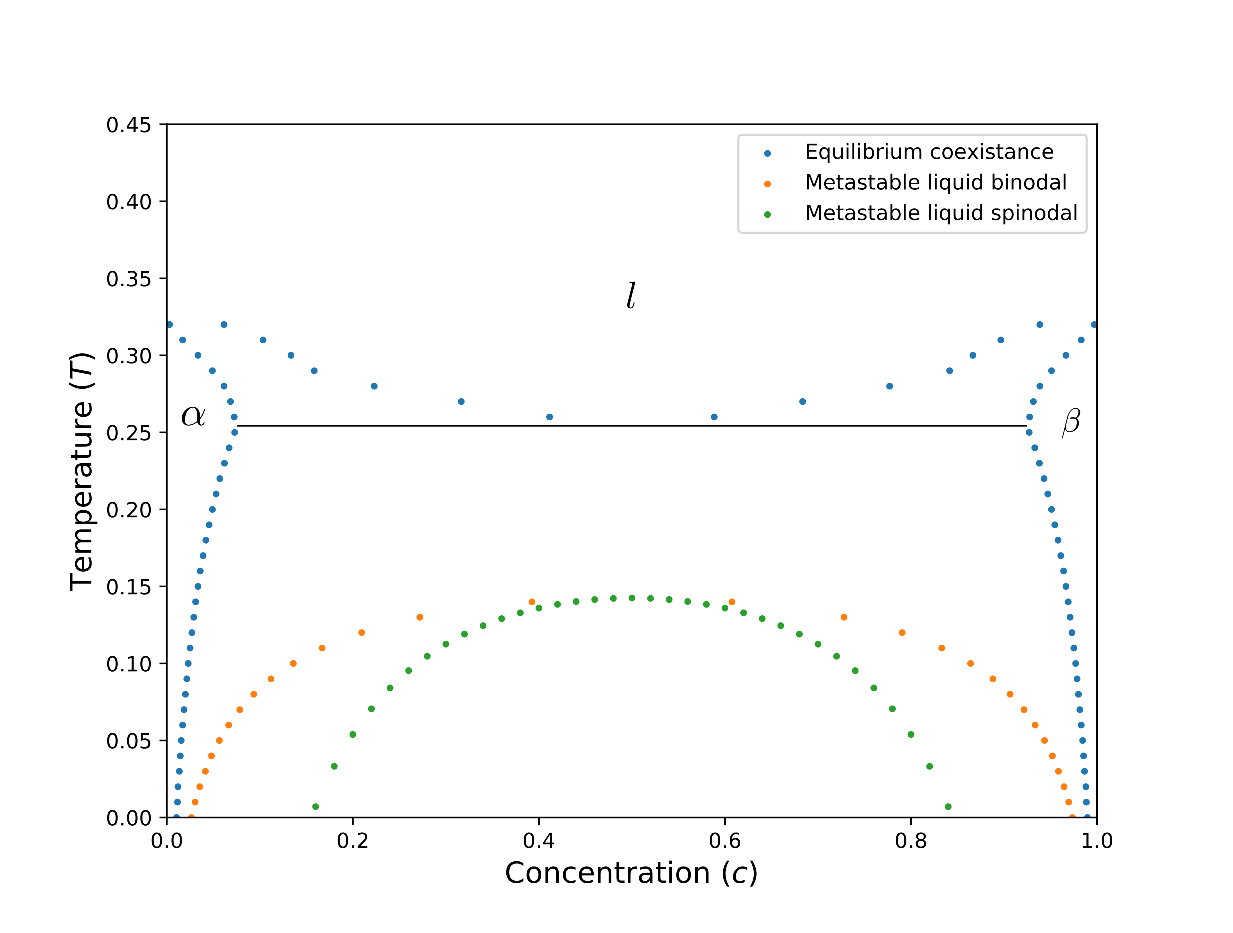
\includegraphics[scale=0.5]{eutectic}
	\caption{\label{eutectic} Eutectic phase diagram triangle $\alpha$ and $\beta$ phases. The free energy parameter are $\eta = 2$, $\chi = 1$, $\omega=0.30$, $\epsilon_0 = 3$ and $T_c = 0.01$. The parameters of the structure functions are $\alpha_{10\alpha} = \alpha_{10\beta} = 0.8$, $k_{10\alpha} = 2\pi$, $k_{10\beta} = 4\pi/\sqrt{3}$ and $T_0 = 1$}
\end{figure}


\subsection{Syntectic Phase Diagram}

Our regular model also allows for the study of a variety of invariant binary reactions that, to date, have not been studied using phase field crystal models. One such reaction is the syntectic reaction. 

The syntectic reaction, $l_1 + l_2 \rightarrow \alpha $, consists of solidification at the interface of two liquids. We can achieve this with our model by setting the spinodal temperature, $T_c$, sufficiently high and producing a density-density correlation function that is peaked at a concentration below the spinodal. This can be done by choosing a window function that is centered about an intermediate concentration, $c_\alpha$ of the solid phase, $\alpha$. 

\begin{equation}
  \chi(c) = e^{- \f{(c - c_\alpha)^2}{2 \alpha_c}}
\end{equation}

The resulting correlation function for a hexagonal lattice in two dimensions, for example, would be,

\begin{equation}
  \tilde{C}_{nn}(k; c) = e^{-\f{(c - c_\alpha)^2}{2 \alpha_c}} e^{-\f{T}{T_0}} e^{-\f{(k - k^\prime)^2}{2\alpha^2}}
\end{equation}
A phase diagram that produces a syntectic reaction with an appropriate choice of parameters can be seen in Fig. \ref{syntectic}.

\begin{figure}
	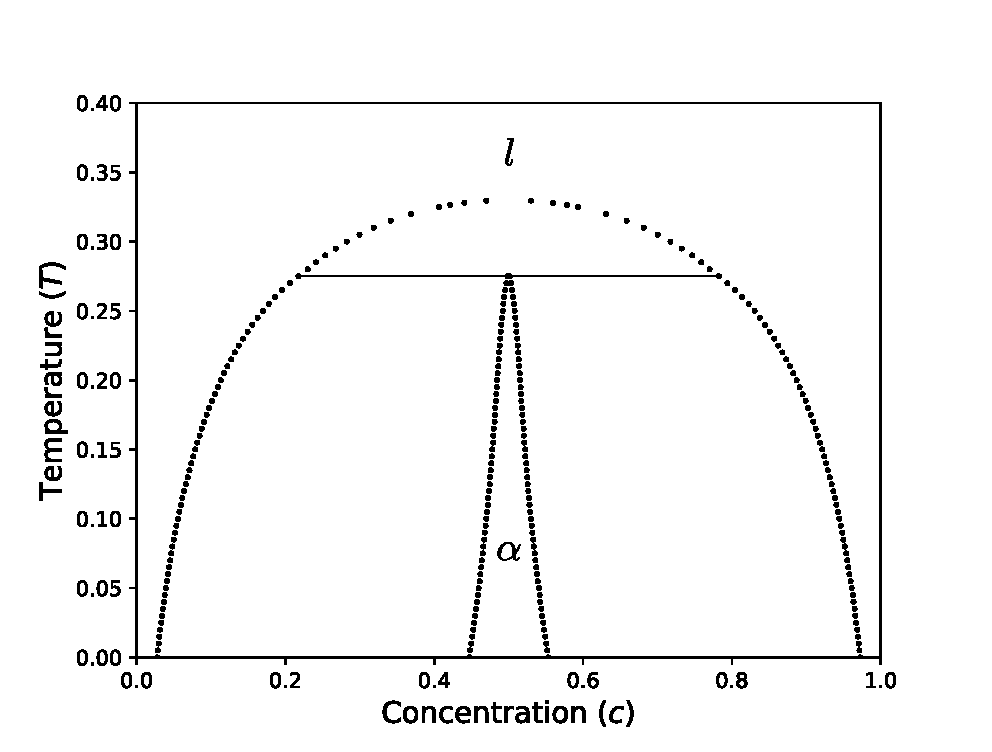
\includegraphics[scale=0.5]{syntectic.eps}
	\caption{\label{syntectic} Phase Diagram of Syntectic Alloy with a hexagonal $\alpha$ phase. The free energy parameters are $\eta=2$, $\chi=1$, $\omega=0.3$, $\epsilon_0 = 10$ and $T_c=0.35$. The parameters for the structure function are $\alpha_{10\alpha} = 0.8$, $k_{10\alpha} = 2\pi$ and $T_0 = 1$}
\end{figure}

\subsection{Monotectic Phase Diagram}

The monotectic reaction is another invariant binary reaction that has not previously been studied using PFC models. The monotectic reaction, $l_1 \rightarrow \alpha + l_2$, consists of decomposing liquid into a solute poor solid and solute rich liquid. To model a monotectic using our regular model we hypothesize a solid phase at $c=0$ and set the spinondal temperature higher than the solidification temperature. To achieve this we use a window function peaked around $c = 0$,

\begin{equation}
    \chi_\alpha(c) = e^{-\f{c^2}{2\alpha_c^2}}.
\end{equation}
Again considering a simple hexagonal lattice for the $\alpha$ phase, we can produce a phase diagram with a monotectic reaction with an appropriate choice of parameters as in Fig. \ref{monotectic}. 
\begin{figure}
	\includegraphics[scale=0.5]{monotectic.eps}
	\caption{\label{monotectic} Phase Diagram of Monotectic Alloy with hexagonal $\alpha$ phase. The free energy parameters are $\eta = 2$, $\chi=1$, $\omega=0.3$, $\epsilon_0 = 10$, $T_c = 0.35$ and $c_0 = 0.75$. The parameters for the structure function are $\alpha_{10\alpha} = 0.8$, $k_{10\alpha} = 2\pi$ and $T_0 = 1$ and the parameter for the window function is $\alpha_c = 0.4$}
\end{figure}

\subsection{Precipitation from Solution}

We can also model precipitation of nanoparticles from solution. Precipitation from solution is a typical synthesis technique for gold and silver nanoparticles [cite]. Recent work by [cite nature chem paper] shows that a metastable spinodal may be playing an important role in the growth and nucleation of gold nanoparticles under certain diffusive circumstances.

\begin{figure}
	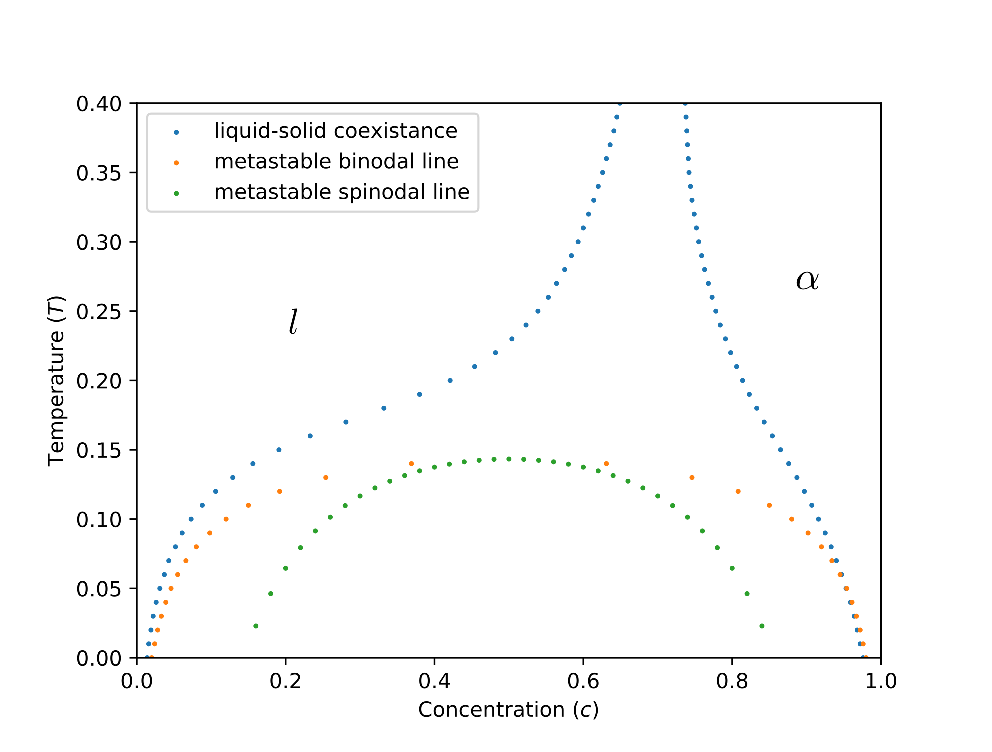
\includegraphics[scale=0.3]{solution.eps}
	\caption{\label{precip} Phase Diagram of Solution}
\end{figure}

\section{Application}

\subsection{Non-classical nucleation pathways of precipation from solution}

\subsection{Anomolous growth of nanoparticles}

\bibliography{references/references.bib}

\end{document}
